\documentclass[12pt,a4paper]{article}

\usepackage[croatian]{babel}
\usepackage[utf8]{inputenc}
\usepackage[hyphens]{url}

\usepackage{graphicx}

\usepackage[margin=2cm]{geometry}
\usepackage[colorlinks=true,urlcolor=black]{hyperref}
\pagenumbering{gobble}

\begin{document}
	\title{Očitavanje senzorskih podataka korištenjem računala Raspberry Pi 3}


	\date{\vspace{-5ex} 3. travnja 2017.}
	\maketitle

	\tableofcontents
	\newpage

\section{Uvod}
Ovaj će seminarski rad obraditi problematiku korištenja računala Raspberry Pi 3 za prikupljanje podataka sa senzora. Ukratko će se opisati sklopovska arhitektura računala Raspberry Pi 3 te pripadajuća programska podrška, uz nekoliko primjera korištenja. \\ \par
Kao vrlo pristupačno malo računalo, Raspberry Pi je vrlo popularan kao ugradbeno računalo, a budući da ugradbena računala vrlo često za svoj rad koriste raznolike senzore, za ovaj će rad biti ključno razumjeti osnovne principe povezivanja senzora i računala, uzimajući u obzir sklopovski i programski aspekt. Shodno tome, bit će izložen kratak opis nekoliko akcelerometara, u funkciji senzora za mjerenje vibracija, i mikrofona, poglavito u funkciji senzora glasnoće. \\ \par
Ukratko će se opisati neke od dostupnih biblioteka i programskih okvira namijenjenih za rad sa senzorima, s naglaskom na već spomenute akcelerometre i mikrofone. Konačno, bit će pokazan i jednostavan primjer programskog koda za očitavanje podataka sa senzora uz prateći primjer vizualnog prikaza senzorskih podataka. \\
\newpage


\section{Raspberry Pi}

Raspberry Pi je serija malih računala razvijanih od strane zaklade Raspberry Pi Foundation. Odlikuju ih niska cijena, dobre performanse s obzirom na cijenu, pristupačnost i lako korištenje te male fizičke dimenzije. Programska je podrška otvorena i vrlo dobro dokumentirana, a zajednica ljudi koji koriste Raspberry Pi je velika, pristupačna i konstruktivna. \\
\par
U trenutku pisanja su dostupni Raspberry Pi 1, 2 i 3, te minijaturni Raspberry Pi Zero. U nastavku će rada riječ biti o Raspberry Pi 3 inačici, koja se vidi na Slici \ref{fig:rpi3}, a bit će oslovljena kao "RPi3".
\begin{figure}[h!]
  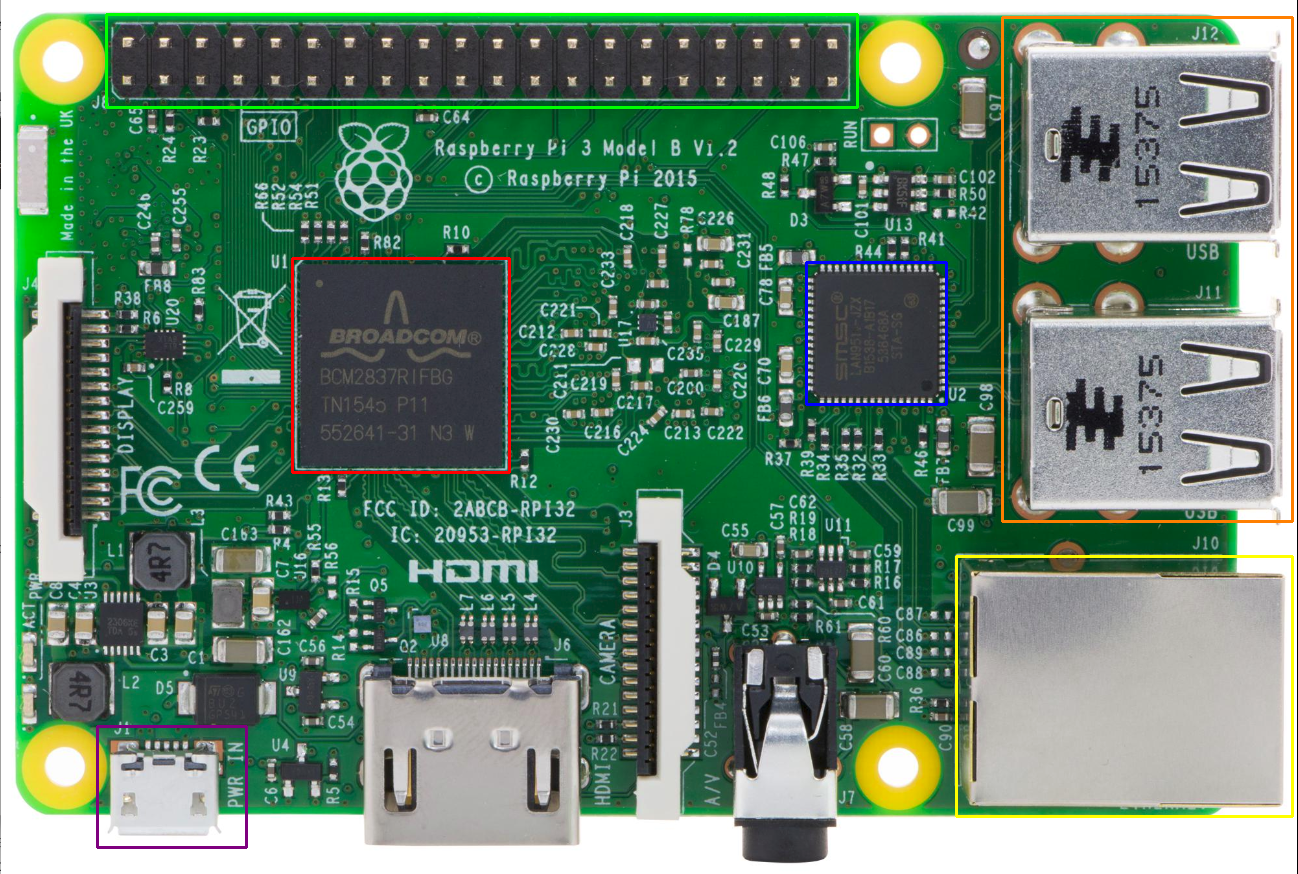
\includegraphics[width=\linewidth]{slike/rpi3_color.png}
  \caption{Raspberry Pi 3B.}
  \label{fig:rpi3}
\end{figure}

	\subsection{Sklopovlje}
		\paragraph{Glavni čipovi} % (fold)
		\label{par:main_chips}
		
		% paragraph glavni_cipovi (end)
		Glavne procesne jedinice nalaze se u čipu Broadcom BCM2837, koji je na slici označen crvenim pravokutnikom. Riječ je o tzv. \textit{System-on-Chip} (SoC) čipu koji sadrži:
		\begin{itemize}
			\item CPU - 64-bitni ARMv8 Cortex A53 s četiri jezgre na 1.2 GHz,
			\item GPU - VideoCore IV na 400 MHz.
		\end{itemize}

		\par Taj je SoC spregnut s radnom memorijom s druge strane tiskane pločice. Riječ je o LPDDR2 SDRAM memoriji, s kapacitetom od 1 GB.

		\par Za bežičnu je komunikaciju zadužen procesor osnovnog pojasa (engl. \textit{baseband processor}) BCM43438, također od tvrtke Broadcom, koji podržava WiFi i Bluetooth 4.1 protokole. Smješten je na stražnjoj strani pločice, a spregnut je s antenom na prednjoj strani.

		\par Konačno, SMSC LAN9514 (na slici uokviren plavom bojom) vrši funkciju USB čvora i Ethernet upravljača. Povezan je s procesorom jednom USB vezom, pa sa svakim od četiri USB priključka, te s Ethernet priključkom procesor komunicira preko te USB veze.

		\paragraph{Ulazno-izlazni priključci} % (fold)
		\label{par:IO_ports}
		
		% paragraph ulazno_izlazni_priključci (end)
		Kao i svako drugo računalo, i RPi3 bi bio prilično beskoristan bez mogućnosti komunikacije s vanjskim svijetom. Naravno, na njemu postoji mnoštvo ulazno-izlaznih sučelja, a način na koji su ona izvedena je uvelike zaslužan za takvu popularnost ovog računala. Za ovaj seminar najvažniji priključci označeni su na Slici \ref{fig:rpi3}, a u nastavku je dan pregled tih sučelja:
		\begin{itemize}
			\item Četiri USB 2.0 priključka [narančasti pravokutnik],
			\item Jedan Ethernet priključak [žuti pravokutnik],
			\item Jedan microUSB priključak - samo za napajanje, ne i za komunikaciju [ljubičasti pravokutnik],
			\item Četrdeset ulazno-izlaznih pinova opće namjene (GPIO - \textit{General Purpose Input/Output}) [zeleni pravokutnik],
			\item Audio priključak i HDMI izlaz
			\item Poseban priključak za službenu Raspberry Pi kameru
			\item Poseban \textit{display} priključak
		\end{itemize}

		\par Od posebne su važnosti za ovaj rad GPIO pinovi. Oni, su, naime, ključni za komunikaciju sa senzorima koji će biti razmotreni kasnije u radu. Omogućuju najčešće korištene \textit{low-level} protokole za sklopovsku komunikaciju: I$^2$C, TTL i SPI. Naravno, sadrže i pinove za napajanje i uzemljenje sklopova, kao i pinove s ponašanjem definiranim od strane korisnika.

	\subsection{Programska podrška}
	\subsection{Primjeri korištenja}
\newpage
% Riječ je, naime, o tzv. \textit{System-on-Chip} (SoC) računalu, pa je cijelo računalo veliko kao bankovna kartica. Iz navedenih se razloga Raspberry Pi računala najčešće susreću u dva konteksta:
%\begin{itemize}
%	\item u edukativnim projektima (pristupačnost i cijena)
%	\item u ugradbenim sustavima (male dimenzije i cijena)
%\end{itemize}

\section{Senzori}
	\subsection{Akcelerometri}
		\subsubsection{ADXL345}
		\subsubsection{MMA8451}
		\subsubsection{LIS3DH}

	\subsection{Mikrofoni}
		\subsubsection{placeholder}
\newpage
\section{Pregled dostupnih programskih okvira}

\newpage
\section{Primjeri}
	\subsection{Programski kôd}
	\subsection{Očitani podaci}

\newpage
\section{Zaključak}

\newpage
\section{Literatura}

\begin{itemize}
	\item Raspberry Pi službene stranice: \url{https://www.raspberrypi.org/}
	\item ADXL345: \url{https://learn.adafruit.com/adxl345-digital-accelerometer}
	\item MMA8451: \url{https://learn.adafruit.com/adafruit-mma8451-accelerometer-breakout/wiring-and-test?view=all}
	\item LIS3DH: \url{https://learn.adafruit.com/adafruit-lis3dh-triple-axis-accelerometer-breakout/downloads?view=all}
	\item Zvučni senzori: \url{https://www.sunfounder.com/learn/sensor-kit-v2-0-for-raspberry-pi-b-plus/lesson-19-sound-sensor-sensor-kit-v2-0-for-b-plus.html}
\end{itemize}

\end{document}